%
% $Id: ch02_relatedwork
%
%   *******************************************************************
%   * SEE THE MAIN FILE "AllegThesis.tex" FOR MORE INFORMATION.       *
%   *******************************************************************
\chapter{Related Work}\label{ch:relatedwork}

 Automated and semi-automated analysis of source code has remained a topic of intense research for more than 30 years \cite{Binkley}. It helps programmers to work more efficiently and enforces rules to use the same programming patterns. This paper will explore and compare the effectiveness of some of these tools. In this chapter, some additional tools are mentioned 
 


\section{Java Visualizer}

\begin{figure}[htbp]
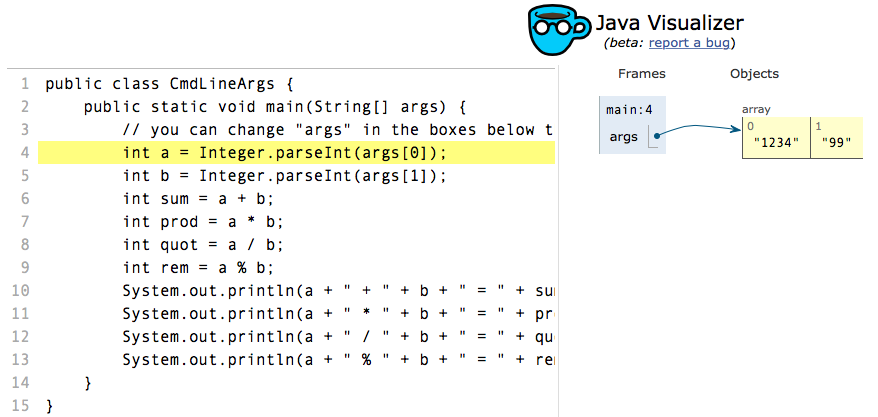
\includegraphics[scale=0.5]{JavaVisualizer}
\caption{Java Visualizer used to go through a Java program line by line}
\label{fig:jv}
\end{figure}

In Table \ref{fig:jv}, the Java Visualizer is used to go through a Java program line by line and provide a visualization of the program steps on the right hand side.

\section{Jlint}
%Jlint
Jlint is a static code analyzer that checks Java source code to attempt to find bugs. Throughout the code, it looks for inconsistencies and synchronization problems. It is done by performing data flow analysis and building a lock graph. Jlint is a simple but highly effective static analyzer that checks Java programs for several common errors, such as null pointer exceptions and overflow errors \cite{artho_havelund}.
%Applying Jlint to Space Exploration Software
The original version Jlint1 was just a Java program checker that could check packages in an automated manner. Jlint1 was extended to Jlint2 to fully support synchronization. \cite{Artho:2001:ASA:872024.872575}.
%Applying Static Analysis to Large-Scale, Multi-Threaded Java Programs
\section{Bandera}
Bandera is an integrated collection of program analysis and transformation components \cite{Corbett:2000:BEF:337180.337234}. %Bandera: Extracting Finite-state Models from Java Source Code
Bandera takes Java source code and outputs a program model in the input language for several existing verification tools \cite{Corbett:2000:BEF:337180.337234}.

Bandera evaluates the model by checking the Java source code. It provides tool to support definition and managing collections of requirements \cite{Corbett:2000:BSI:337180.337625}.
%Bandera: A Source-level Interface for Model Checking Java Programs

\section{ESC/Java2}
%ESC/Java 2
ESC/Java2 (Extended Static Checker for Java) is the main (extended) static checker for the JML (Java Modeling Language) \cite{chalin_kiniry_leavens_poll}. The purpose of the extension is to include extra constructs for specifying an object-oriented module such as frame properties, data groups, and ghost and model fields \cite{chalin_kiniry_leavens_poll}.
%Beyond Assertions: Advanced Specification and Verification with JML and ESC/Java2

At first, it was an experimental compile-time program checker that found common programming errors. The checker is powered by verification-condition generation and automatic theorem-proving techniques \cite{Flanagan:2002:ESC:512529.512558} \cite{Flanagan:2002:ESC:543552.512558}.
%Extended Static Checking for Java

\section{Summary of Related Work}
There are a number of tools that assist programmers in working more effectively. Three of these have been researched in this paper, but apart from these there are many other tools. The tools that are presented in this paper may not detect a possible bug (false negative) or may highlight a point in the source code that may not be the bug (false positive). My proposed study is to evaluate three tools for four Java programs that have been written to include a bug. This will provide Java programmers information about tools to assist in detecting logic based bugs.


%A typical second chapter deals with a survey of the literature
%related to the thesis topic. The subsections may be organized in whatever
%manner seems best suited to the material---chronological, or by topic, or
%according to some other criteria (e.g., primary versus secondary resources).
%The examples given in the sections in this chapter are nonsensical in content;
%they are provided merely to give examples of citing bibliographic references.
%Resources should be cited by author name(s), not by title.
%There should be a space between the square brackets of a citation and
%any preceding words. Thus, ``Smith and Jones[17]'' is wrong; ``Smith and
%Jones [17]'' is correct. If the citation is at the end of a sentence, the
%period goes after the brackets (``Johnson [23].'', not ``Johnson. [23]'').


%The earliest work done in widget software is described in the seminal 1986
%paper by Smith and Jones \cite{SmithJones86}. Using a networked array of
%high-performance computers they demonstrate that widgets with $k$ degrees
%of freedom can be simulated in time proportional to $k\log^2k$. At the
%heart of their demonstration is an algorithm for re-encabulating the widgets
%using a lookup table that can be updated in real time, assuming that
%the widgets are non-orthogonal. The question of simulating orthogonal widgets
%is left open, but the authors conjecture that orthogonality will add at
%ost another factor of $k$ to the performance upper bound.


%A number of papers \cite{blum67,damon:95,zobel:97} deal with issues
%that are peripheral to the orthogonal case, but Dio\c{s}an and Oltean
%were the first to tackle it directly.
%In their 2009 paper \cite{diosan09}, 
%Dio\c{s}an and Oltean apply evolutionary techniques to
%the orthogonal widget case, obtaining empirical results that suggest
%an efficient algorithm might be at hand. Their
%approach is characterized by the use of a genetic algorithm to evolve other,
%more problem-specific evolutionary algorithms. 

